\documentclass[tikz,border=10pt]{standalone}
\usepackage{tikz}
\usetikzlibrary{arrows.meta, positioning}

\begin{document}
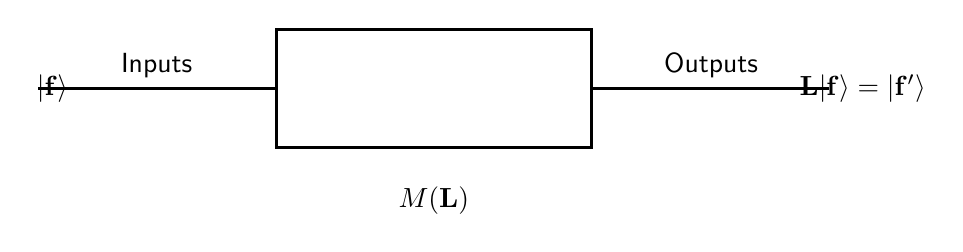
\begin{tikzpicture}[>=Stealth, font=\sffamily]

% Define nodes
\node[draw, very thick, minimum width=4cm, minimum height=1.5cm, label={[yshift=-1em]below:$M(\mathbf{L})$}] (box) {};
\node[left=of box, anchor=east, xshift=-1.5cm] (input) {$|\mathbf{f}\rangle$};
\node[right=of box, anchor=west, xshift=1.5cm] (output) {$\mathbf{L}|\mathbf{f}\rangle = |\mathbf{f}'\rangle$};

% Add horizontal lines and labels
\draw[very thick] (box.west) -- ++(left:3cm) node[midway, above] {Inputs};
\draw[very thick] (box.east) -- ++(right:3cm) node[midway, above] {Outputs};

% Draw horizontal line through inputs
\draw (box.west) -- ++(left:3cm);

% Draw horizontal line through outputs
\draw (box.east) -- ++(right:3cm);

\end{tikzpicture}
\end{document}